Apply the RBF-PS method to solve the heat equation and Helmholtz equation (i.e., the eigenvalue problem for the 
Laplacian) in 1D.

\begin{solution}
    We apply the RBF-PS method to solve PDEs by searching for an approximate solution of the form

    \begin{equation}\label{eq:rbf-approximation}
        U(x) = \sum\limits_{j=1}^N c_j \phi(\lVert \bm{x} - \bm{x}_j \rVert)
    \end{equation}

    where $\phi$ is a radial basis function. We then solve for the appropriate coefficients $c_j$ by enforcing the PDE 
    at collocation points $\bm{x}_j$. In particular, for a particular linear differential operator $\mathcal{L}$,
    the associated operator matrix $L$ is given by

    $$
    L = A_{\mathcal{L}} A^{-1}
    $$

    where $A$ is the RBF matrix given in Problem 1. For the second spatial derivative, we have

    $$
    \mathcal{L} = \frac{\partial^2}{\partial x^2}
    $$

    so that each entry of $A_{\mathcal{L}}$ is given by

    $$
    (A_{\mathcal{L}})_{ij} = \frac{\partial^2}{\partial x^2} \phi(\lVert \bm{x} - \bm{x}_j \rVert)\bigg|_{\bm{x} = \bm{x}_i}.
    $$

    We utilize a Gaussian RBF so that

    $$
    (A_{\mathcal{L}})_{ij} = 2 \epsilon^2 \left(2 \epsilon^2 r_{i,j}^2 - 1 \right) e^{-(\epsilon r_{i,j})^2}, \quad r_{i,j} = \lVert \bm{x}_i - \bm{x}_j \rVert.
    $$

    We now apply this matrix to the 1D heat equation with Dirichlet boundary conditions and sinusoidal initial 
    condition on $\Omega = [0, 1]$ where $t \in [0, 1]$: 
    
    $$
    u_{xx} = u_t,  \quad u(x, 0) = \cos{\frac{\pi x}{2}}, \quad \text{and} \quad u(0, t) = u(1, t) = 0. 
    $$

    We enforce boundary conditions by extending $A_{\mathcal{L}}$ appropriately to enforce collocation at the boundary 
    points. For time stepping, we utilize a forward Euler scheme. This algorithm is implemented in 
    \texttt{problem\_3i\_heat.m}, and results are shown in Figure \ref{fig:problem_3i_heat}.
    
    \begin{figure}[h]
        \centering
        \begin{subfigure}{0.45\textwidth}
            \centering
            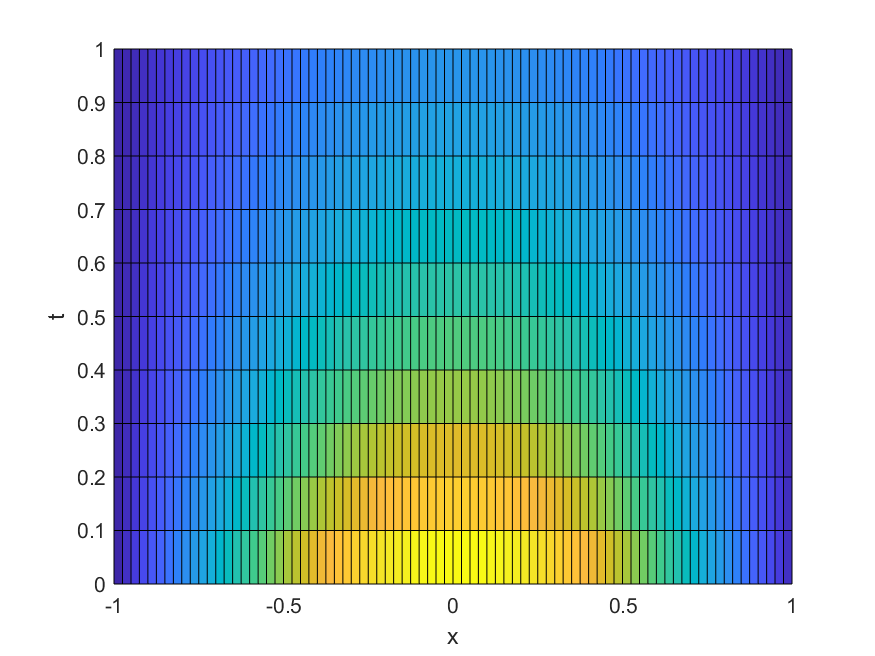
\includegraphics[width=\textwidth]{problem_3i_heat_2d.png}
            \caption{2D plot of 1D heat equation solution.}
            \label{fig:problem_3i_heat_2d}
        \end{subfigure}
        \begin{subfigure}{0.45\textwidth}
            \centering
            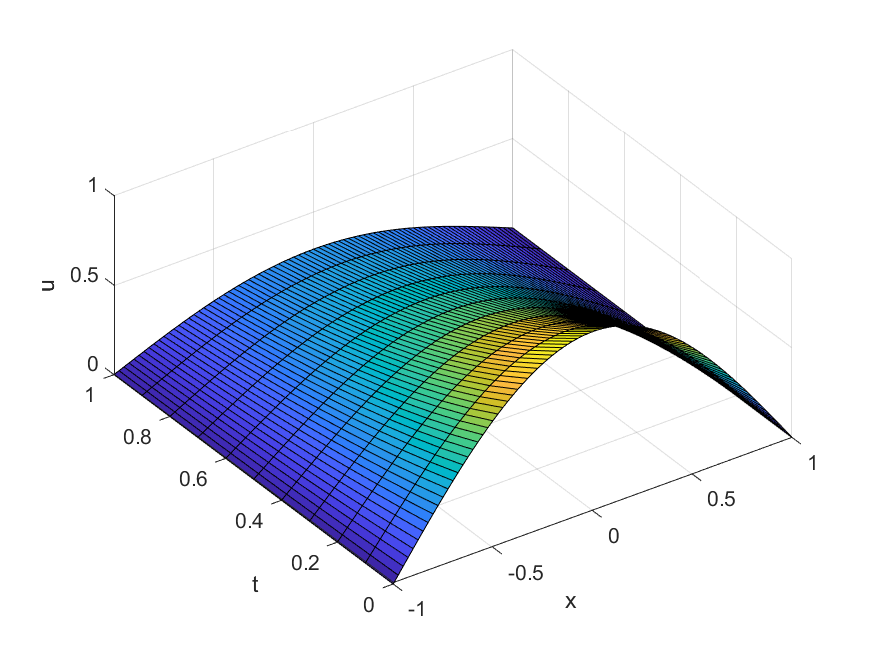
\includegraphics[width=\textwidth]{problem_3i_heat_3d.png}
            \caption{3D plot of 1D heat equation solution.}
            \label{fig:problem_3i_heat_3d}
        \end{subfigure}
        \caption{Solution to the 1D heat equation using the RBF-PS method.}
        \label{fig:problem_3i_heat}
    \end{figure}

    \pagebreak
    We now apply the RBF-PS method to solve the Helmholtz equation in 1D with Dirichlet boundary conditions on 
    $\Omega = [-1, 1]$:

    $$
    u_{xx} = k^2 u \quad \text{and} \quad u(-1, t) = u(1, t) = 0. 
    $$

    We move everything to the left hand side to find the associated eigenvalue problem:

    $$
    \left( \mathcal{L} - \lambda I \right) u = 0.
    $$

    where we let $\lambda = k^2$ for convenience. The solution to this system is therefore given by the eigenvectors of 
    $\mathcal{L}$; in the RBF-PS case, this reduces to computing the eigenvalues and eigenvectors of the (second-order) 
    differentiation matrix $A_{\mathcal{L}}$. We compute the eigenvalues and plot corresponding eigenvectors in 
    \texttt{problem\_3i\_helmholtz.m}. The exact eigenvalues are given by 
    
    $$
    \lambda_j = \frac{j^2 \pi^2}{L^2}
    $$
    
    where $L = 2$ is the length of the domain. The output of \texttt{problem\_3i\_helmholtz.m} is given below:

    \begin{figure}[h]
        \begin{verbatim}
            
        \end{verbatim}
        \caption{Output of \texttt{problem\_3i\_helmholtz.m}.}
        \label{fig:problem_3i_helmholtz_output}
    \end{figure}

    \pagebreak
    Plots of the eigenvectors and eigenvalues are shown in Figure \ref{fig:problem_3i_helmholtz_eig}.

    \begin{figure}[h]
        \centering
        \includegraphics*[width=\textwidth]{problem_3i_helmholtz.png}
        \caption{Eigenvalues and eigenvectors of second derivative RBF matrix.}
        \label{fig:problem_3i_helmholtz_eig}
    \end{figure}
\end{solution}